\section{Introduction}

\subsection{Background}

Fault-tolerant constructions take ideal quantum circuits and establish their logical equivalence such that they endure fault occurrences. Their efficiency is typically measured by the amount of additional resources – qubits, computation time, range connectivity, etc. – required by the resulting circuit, beyond the scope of theoretical discussion; those parameters translate into the machine complexity and energy cost required to run the circuits. Minimizing overheads brings quantum computing applications closer to the near future.

Since the introduction of the quantum threshold theorem \cite{aharonov1999faulttolerant}, which showed that quantum fault tolerance is in principle feasible, the main effort in subsequent work has focused on reducing the additional qubit overhead. A line of work has led to a constant-factor overhead in qubits, first in the instant-classical computation model \cite{gottesman2014faulttolerant}, then in the standard circuit model \cite{grospellier:tel-03364419}, \cite{Fawzi_2018}, \cite{ nguyen2025quantumfaulttoleranceconstantspace}. Yet, although the best qubit overhead was reached, the depth overhead was only slightly improved from poly-logarithmic to logarithmic \cite{ nguyen2025quantumfaulttoleranceconstantspace}. In fact, it seems that the same means that are used to reduce the qubit overhead are the ones that challenge reducing the depth overhead.    

A key concept for reducing qubit overhead is to encode qubits with a high-rate quantum LDPC code.  For those codes, except for the control-not, there are no known gates that can be realized in constant depth; furthermore, since the structure of the codes is relatively complicated – based on the skeletons of expander graphs - it seems hard to look for realizations of their logical operators. Without a constant-depth realization of logical operators, any construction that doesn't interfere with the order of the logical operations would admit a non constant-depth overhead. 

Contrary to high-rate LDPC codes, topological error codes have a geometrical image that is well understood and, as a result, a wide range of works suggest efficient realization of their logical operators. For example, consider the 3D-color code \cite{Bombín_2015}, fold-transversal gates on the surface code \cite{Breuckmann_2024}, and realization of the Clifford group on the 2D Toric \cite{guernut2024faulttolerantconstantdepthcliffordgates}.

Another branch of work, whose primary goal was to show that the embedding dimension of the computation can be reduced to 2D \cite{Balasubramanian_2026}, and more recently \cite{dünnweber2026quantummemoryautonomouscomputation}, uses topological codes as the main error correction code. Those constructions simplify the hardware realization; they suggest that quantum computers can be implemented by nearest-neighbor interactions automata - what is believed to be easier to develop. Yet, as in the threshold theorem \cite{aharonov1999faulttolerant}, and in contrast to the works that use high-rate LDPC codes, they rely on a hierarchical correction cycle whose execution time grows with system size. Hence, even though those directions have the potential to overcome the non-constant depth overhead per gate, it seems that the correction cycle imposes a barrier for them to come up with a constant factor in depth-overhead construction. 

\subsection{Stating Our Results}
In this work, we present a fault-tolerance construction that uses the 4D Toric code and has a constant-depth 'correction' cycle. Or in other words, a construction uses a relatively simple code, yet doesn't admit the cost of hierarchical correction cycle. 

The computation model we consider is quantum circuits subject to \textit{local-stochastic noise}, where only qubits are subjected to the noise, while classical bits are non-noisy. Classical computation is allowed, and the classical depth matters. Namely, at each time unit, only a constant depth of classical computation can be done.  Local stochastic channel is defined to act such that the probability of any subset of locations $S$ (space-time coordinates), which is picked prior to the channel's action, being affected decays exponentially with the subset size. 
\begin{definition}[Local stochastic noise channel]
  Let $p\in(0,1)$. We say that the noise channel $\mathcal{N}_{\mathcal{E}}$ is \textit{local stochastic with rate $p$} if for every finite set of locations $S\subset \mathbb{N}\times \mathbb{N}$,
  \begin{equation*}
    \begin{split}
      \prbm{S\subset \operatorname{Loc}(\mathcal{E})}{\mathcal{E}\sim \mathcal{N}_{\mathcal{E}}}
      \le p^{|S|}.
    \end{split}
  \end{equation*}
\end{definition}

For circuits $\tilde{C}$ and $C$, we say that $\tilde{C}$ simulates $C$ with probability $p$ if, when one stops a noisy run of $\tilde{C}$ at a midpoint, they can, with probability $p$, recover by non-noisy operation an 'image' of a midpoint in the running of $C$, and if stopping at the last time point of $\tilde{C}$ enables recovery of the 'image' of $C$ at the end of its run. We proved the following theorem: 
\begin{theorem}[Informal]
There exists a constant $p_{0} \in (0,1)$ such that for any local stochastic noise channel $\mathcal{N}_{\mathcal{E}}$ with rate $p < p_{0}$, a quantum circuit $C$ with depth $\mu$ and width $w$, and a big enough integer $n$, there exists a 'logical equivalence' circuit $\tilde{C}$ with depth $\Theta(\mu n)$ and width $\Theta((w + \mu) n)$ that simulates $C$ with probability:
\begin{equation*}
  \begin{split}
    1 -   \Theta \left( \text{poly}(w,\mu,n) \right)  p^{\Theta(n^{\frac{1}{4}})} 
  \end{split}
\end{equation*}
Furthermore, $\tilde{C}$ has the following two properties:
\begin{enumerate}
  \item After a short initialization stage (at depth $\Theta(\log n)$), the qubits are encoded in the $n$-length 4D Toric code.
  \item An error correction cycle takes $O(1)$ depth, and the gates in each correction cycle don't depend on time. In particular, if $C$ is the identity circuit, then after the initialization stage, the layers in $\tilde{C}$ are the same.
\end{enumerate}
  \end{theorem} 
  As mentioned earlier, both code simplicity and constant depth have already been achieved: the former as part of the quantum automation line of work, and the latter through the use of high-rate error correction codes. However, this is the first construction to achieve both simultaneously. \Cref{fig:comapreresults} summarizes and compares the different works:

\newcommand{\tcite}[1]{\hfill\cite{#1}}
%\scalebox{0.8}{
  \begin{table}[h]
    %\centering
    %\setlength{\tabcolsep}{4pt}
    {
      \footnotesize
      \begin{tabular}{l p{4cm} p{3cm} p{2cm} p{3cm}}
        \toprule
        {\sc Works Line }  &   	\textsc{Error correction \newline code}  &   \textsc{Constant-depth \newline correction \newline cycle}   &   \textsc{Depth/qubit \newline overhead }  &  \textsc{Ref}    \\
        \midrule
        {\sc Concatenation }   & Concatenation of \newline fixed length code  & \ding{55}  & $f(x)$  & \cite{aharonov1999faulttolerant} \\
        {\sc High-rate }       & Quantum expanders/ good QLDPC &  \ding{51}     & $f(x)$ &  \cite{grospellier:tel-03364419}, \cite{Fawzi_2018}, \cite{nguyen2025quantumfaulttoleranceconstantspace}  \\
        {\sc Quantum Automata } & 2D-Toric code    & \ding{55}        & $f(x)$ &  \cite{Balasubramanian_2026}, \cite{dünnweber2026quantummemoryautonomouscomputation}  \\
        {\sc Ours}             & 4D-Toric code    & \ding{51}                            & $f(x)$ & \\
        \bottomrule
      \end{tabular}

    }
    \caption{\label{fig:comapreresults} Comparing different types of works on fault-tolerance. }
  \end{table}


\subsection{Discussions, Applications, and Further Directions}
Our result can be understood as follow: when the qubit overhead is not a consideration, it means that the 4D Toric code is as good as the good quantum LDPC / Hyperproduct code. That translates to the two following applications: 
\begin{enumerate}
    \item New approach for quantum fault tolerance: With the assistance of resource states and gate teleportation, we obtain a fault-tolerant construction with logarithmic depth overhead. Our proof is inherently different from prior works, describes in higher resolution the expected error, and might be used as a springboard for a constant depth overhead construction.   
    \item Memory in the circuit model: Protecting a 4D Toric encoded state for an exponentially long time is achieved by performing the same operation at each time unit, suggesting that the 4D Toric code is a promising candidate for memory in the circuit model. Combined with evidence that the 4D Toric code also functions as memory in thermal noise models \cite{alicki2008thermalstabilitytopologicalqubit}, and given its relative simplicity, it appears to be a natural choice for real-world memory applications.
\end{enumerate}

\section{Outline of The Proof}
In studying fault tolerance, the typical method is to first distinguish between configurations that can be tolerated and those that cannot. For example, in von Neumann-style proofs \cite{ }, \cite{ }, it is common to track the number of flipped bits; if fewer than half are flipped, the logical states can be recovered. In the work of Aharonov and Ben-Or \cite{aharonov1999faulttolerant}, a logical bit at the $n$ level admits a logical error if at least a constant fraction of the $n-1$ level logical bits that compose it admit an error. In the work of \cite{grospellier:tel-03364419}, a tolerated configuration is one in which all encoded registers can be considered as distributed according to sufficiently weak local stochastic noise. The next step is to demonstrate that from a tolerated configuration, we move with high probability to another tolerated configuration. Each approach presents a challenge: The concatenation method, by definition, requires non-trivial computation at each step. Tracking the number of flipped bits fails almost immediately, as topological error correction codes have sublinear distance when a linear number of bits is expected to be flipped. Preserving the local stochastic noise distribution seems to heavily rely on the expansion properties \cite{grospellier:tel-03364419} of the underlying structure, where for topological codes, we expect to establish a 'spatial' dependence.


In  contrast, Berman and Simon provided a proof that, instead of tracking the dynamics, considers the entire run as a possible outcome, ruling out improbable runs only at the end \cite{Berman}. We outline their idea informally as follows: a logical bit is represented by $n \times n$ bits set on the vertices of the grid. In each correction cycle, the bits determine their value by taking the majority of their north, north-east, and east neighbors, a rule known as Toom's rule. For simplicity, let's ignore the logical operations. Now, given a run, and in particular the set of space-time locations of faults, consider the following directed graph $\mathcal{H} \colonequals (V_{\mathcal{H}}, E_{\mathcal{H}})$ induced by it: 
\begin{enumerate}
  \item If at time $t$, the bit at vertex $v$ diverges relative to the ideal run, then add $(v,t)$ to the vertices. 
  \item If at time $t$, vertex $v$ 'leads' one of its neighbors $u$ to diverge, then connect $(v,t)$ and $(u,t+1)$ by an 'arrow'. 
  \item Connect any two vertices in $V_{\mathcal{H}}$, which are connected to a third by 'arrows', by a 'fork'. 
\end{enumerate}
Notice that the vertices of $\mathcal{H}$ with no incoming arrows correspond to faults; let's call them leaves. Thus, the probability of each running can be bounded by the number of leaves in the induced graph. Their key lemma states that a cluster of flipped bits with a 'perimeter' $s$, connected by arrows, induces a subgraph with at least $\Theta(s)$ leaves. In other words, the probability of a connected component (by arrows) being flipped decays exponentially with its perimeter. 

To generalize, this technice, we have first to well define what error is, a flipping a satabilizer doesn't count as flipping bits. Then, to define an analog for the Toom's rule, proving a lemma that restrict the expansion of error under the applications of the rule, defining a logical operation and their realiztions, and 
\subsection{The Toric Complex and the Infinite Plane}

\subsection{The Intermediate Theorem}

For a adapting   





,  at $O(1)$-depth is our goal, we have to give up a full corrections,  it seems   ..,   In  \cite{GACS1988125}, the 

That can be thought as an adaptation  Gacs and Reif ideas \cite{GACS1988125}, Where the $n$-logical bit corresponds to colony, in their approach corrections done via the Toom's rule which is uniform for all the bits. 

defined       the logical bit is encoded by a repttion code on the cube/gird, and the analsyis track over subcubes called colonies,    defined as seek if by a reqursive rule: if at least X of its subcubes are seek  ,and define an event where at least a constant factor of bits are flipped as an error. The methodology is to show that, assuming the number of flipped bits is below a certain threshold, after observing noise and executing a correction cycle, the number of resulting flipped bits is expected to remain under the threshold. In the concatenation style of works, it's common to borrow the idea of Gacs and Reif \cite{GACS1988125}, defining a damaged structure (logical error in \cite{aharonov1999faulttolerant} or seek colony in \cite{GACS1988125}) as structures with too many damaged substructures, and showing that in an interval of noisy-computation only less than fraction of substructres are expected to be damaged, only to 'improv the state of substructures with not too many damaged substructures. As the structures and their substructres become at sizes that are comperabile to the system size, the interval also has to do a non trivial computation, in \cite{GACS1988125}) we don't feel it. In  \cite{aharonov1999faulttolerant} we simulate an error correction cycle at one level below, that takes time. 

In both approaches, one ignores 


the classical proofs of Gacs, or in the high-rate works line, One is keeping track over the number of bits that are flipped, and in any turn they show that if the number of fualts are under some ratio, the error correction cycle reduces the error by factor. This is not good for us since a sublinear number of faults are sufficient for bringing into a logical error. And a linear number of errors are expected.



\begin{figure}[htbp]
  \begin{minipage}[c]{0.6\textwidth}
  \centering
\begin{quantikz}
\lstick{$\ket{0}$} & \gate{H} &  & \ctrl{1} &   \\
\lstick{$\ket{0}$} & \gate{H} & \gate{\inr{X}} & \gate{S} &  & \ctrl{1} \\
\lstick{$\ket{0}$} & \gate{H} & \gate{\inr{X}} & \ctrl{1} &  & \targ{} \\
\lstick{$\ket{0}$} & \gate{H} &  & \targ{} & \gate{\inr{X}} & 
\end{quantikz}
\end{minipage}%
  \begin{minipage}[c]{0.3\textwidth}
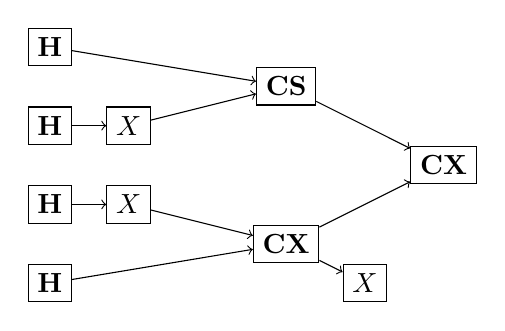
\begin{tikzpicture}
  \node[rectangle,draw] (A)  at (0,3) { $\mathbf{H}$ }; 
  \node[rectangle,draw] (B)  at (0,2) { $\mathbf{H}$ }; 
  \node[rectangle,draw] (C)  at (0,1) { $\mathbf{H}$ }; 
  \node[rectangle,draw] (D)  at (0,0) { $\mathbf{H}$ }; 
  \node[rectangle,draw] (E) at (1,2) { $\inr{X}$ } ; 
  \node[rectangle,draw] (F) at (1,1){ $\inr{X}$ }  ; 
  \node[rectangle,draw] (G)  at (3,2.5) { $\mathbf{CS}$ }; 
  \node[rectangle,draw] (H)  at (3,0.5) { $\mathbf{CX}$ }; 
  \node[rectangle,draw] (I)  at (4,0) { $\inr{X}$ }; 
  \node[rectangle,draw] (J)  at (5,1.5) { $\mathbf{CX}$ }; 
  \draw[->] (B) to (E);
  \draw[->] (C) to (F);
  \draw[->] (A) to (G);
  \draw[->] (E) to (G);
  \draw[->] (F) to (H);
  \draw[->] (D) to (H);
  \draw[->] (H) to (I);
  \draw[->] (G) to (J);
  \draw[->] (H) to (J);
\end{tikzpicture}
\end{minipage}
\caption{  Example of a subjected quantum circuit: the even layers (0, 2, 4) contain the original gates, while the faults are imposed on the odd layers and marked in red. }
  \label{fig:examplecirc}
\end{figure}





\subsection{Description of the Construction}

\subsection{Toom's Contours} 

\section{The Proof in Detail}




